\section{Обзор языка программирования Golang }
Go (также известный как Golang) является статически типизированным компилируемым языком программирования, разработанным на замену ранним языкам системного программирования, таким как C\textsuperscript{++} и Java. 
Созданный Google, Go предоставляет упрощенный синтаксис и мощные инструменты для разработки операционных систем, сетевых сервисов, микросервисов и других распределенных систем \cite{golang}.

Для простоты внедрения данного языка было уделено большое внимание простоте синтаксиса и грамматике языка. 
Многие задачи имеют лишь одно решение средствами языка Go, которое описывается общеизвестными методами парадигм ООП и структурного программирования. 
За счет просты грамматики также достигается высокая скорость компиляции, что положительно сказывается на опыте разработки.

Также для устранения факторов, мешающих разработке, в стандартной поставке языка также предусмотрены инструменты для управления зависимостями и сборки, форматирования кода, синтаксического анализа, генерации и просмотра документации, а также профилирования готовых приложений.

Несмотря на то, что исходные коды языка находятся в общем доступе под свободной лицензией,
процесс разработки по большей части контролируется разработчиками Google и многие решения проходят процесс согласования с проектировщиками языка в лице Кена Томпсона, который участвовал в разработке системы UNIX, Роба Пайка, известного за вклад в развитие операционной системы Plan9, и Роберта Гриземера, который до этого работал над виртуальной машиной V8 для языка JavaScript.

Поэтому, с одной стороны, участие сторонних разработчиков над ядром языка ограничено, поэтому новый функционал принимается с большим количеством обсуждений и согласований, за что язык регулярно критикуют.

Есть мнение, что в текущей реализации языка отрицается многолетний опыт разработки других языков, что отражается в использовании очень простой системы типов, сборщика мусора на поколенческом алгоритме и общей невыразительности базовых синтаксических элементов языка .

С другой стороны, подобный подход гарантирует полную обратную совместимость со старыми программами и маленькое ядро языка с выверенным набором инструментов, которые призваны уменьшать количество дискуссий по поводу вопросов, которые не имеют к разработке прямого отношения: сборка, форматирование, дистрибуция. Что в связке с богатой библиотекой для работы с сетевыми стеками делает Golang хорошим выбором при разработке программ, связанных с веб-разработкой, и послужило причиной выбора данного языка в разработке программного обеспечения для данной работы.

\section{Основные инструменты построения распределенных архитектур}
Одним из ключевых вопросов при построении распределенных архитектур является асинхронная коммуникация
между миросервисами, которая позволяет независимо масштабировать ее компоненты.

Брокер сообщений служит критически важным компонентом при проектировании архитектуры микросервисов, работая как посредник при передаче данных между различными сервисами, 
он позволяет минимизировать прямые связи и обеспечивает ряд ключевых преимуществ, которые облегчают разработку, масштабирование и поддержку сложных микросервисных систем.
Одно из основных преимуществ использования брокера сообщений -- возможность полного разделения различных компонентов системы. 
В архитектуре микросервисов подобное разделение является важным фактором в обеспечении независимости каждого из сервисов. 
Благодаря брокеру сообщений, компоненты в системе не должны прямо общаться друг с другом, что повышает их изоляцию и позволяет им работать независимо. 
Это упрощает процесс обновления или модификации отдельных компонентов, поскольку минимизирует риск сбоев всей системы из-за изменений в одном из сервисов.

Далее, использование брокера сообщений увеличивает надежность системы. Благодаря использованию промежуточного слоя для передачи сообщений, они могут быть надежно сохранены и переданы даже при временных сбоях приема или трансляции. 
Это гарантирует, что важные данные не будут потеряны из-за сбоев или проблем с конкретными сервисами, усиливая отказоустойчивость всей системы.

Помимо этого, брокеры сообщений обеспечивают асинхронную передачу данных. 
Это означает, что система не требует немедленного ответа от сервиса-получателя, что может быть критически важно при высоких нагрузках. 
Брокеры сообщений могут агрегировать сообщения и управлять их доставкой оптимальным образом, обеспечивая более плавную и эффективную работу системы.

На рынке представлено множество различных брокеров сообщений, включая RabbitMQ, Apache Kafka, Google Pub/Sub и AWS Simple Queue Service (SQS). 
Каждый из этих продуктов предлагает различные функции и возможности, такие как надежные очереди сообщений, модели публикации/подписки, устойчивость к ошибкам и многое другое. 
Это позволяет разработчикам выбирать наиболее подходящий брокер сообщений для их конкретных нужд и требований.

В итоге, брокеры сообщений играют ключевую роль в архитектуре микросервисов. Они повышают надежность и устойчивость системы, обеспечивают разделение между сервисами и позволяют более эффективно управлять данными и нагрузкой в рамках сложных микросервисных экосистем.

В данной работе основной акцент делается на Amazon Simple Queue Service (SQS), поскольку он является мощным инструментом для обработки сообщений в архитектуре микросервисов и обладает несколькими ключевыми преимуществами, 
которые делают его привлекательным выбором для различных сценариев использования.

Amazon SQS предлагает высокую надежность благодаря инфраструктуре Amazon. 
Сервис гарантирует доставку сообщения хотя бы один раз, что помогает избежать потери данных. Кроме того, Amazon SQS предлагает очереди с повышенной отказоустойчивостью, которые хранят сообщения на протяжении определенного времени, пока они не будут успешно обработаны получателем.

Amazon SQS легко масштабируется, чтобы обеспечивать эффективную обработку больших объемов данных. 
Благодаря возможности бесконечного расширения, этот сервис может гибко настраиваться для поддержки микросервисов любого размера, чтобы поддерживать высокую производительность без дополнительных усилий с вашей стороны.
Также благодаря тесной интеграции с AWS Identity and Access Management (IAM), Amazon SQS позволяет точно контролировать доступ к очередям сообщений, обеспечивая высокий уровень безопасности. Также доступны функции транзитного шифрования для дополнительной защиты данных.

Вместе с облачной инфраструктурой предоставляются SDK для разных языков, включая AWS Management Console, SDK и CLI. Что позволяет использовать одинаковые семантики и метод API вне зависимости от языка и освобождает от необходимости писать свои клиенты для
взаимодействия с очередью.
Также если вы уже используете другие сервисы от AWS, такие как Lambda, S3 или EC2, использование SQS значительно упрощает интеграцию микросервисов, поскольку все они работают вместе без каких-либо существенных проблем. Использование
S3, например, в качестве промежуточного медиума может позволить передавать сообщения большого размера вне зависимости от отграничений SQS, что представлено в Java SDK для работы с SQS.

Таким образом, Amazon SQS представляет собой отличный выбор для обработки сообщений в архитектуре микросервисов благодаря своей надежности, масштабируемости, безопасности и простоте использования. Благодаря настройке под конкретные потребности и легкой интеграции с другими сервисами AWS, SQS может стать очень ценным активом в микросервисной архитектуре.

При локальной разработке необязательно прибегать к выделению облачных инстансов SQS, а можно воспользоваться сторонними реализациями, которые доступны для развертывания вне облачной инфраструктуры AWS. Примерами подобных решений являются Localstack, Minio, а также официальные образы Amazon
некоторых сервисов, доступных в облаке.

В контексте реализации асинхронного взаимодействия между микросервисами применяются следующий набор методов SDK для языка Go:
\begin{enumerate}
    \item SendMessageWithContext, который отправляет закодированное сообщение в произвольном формате в очередь с адресом QueueUrl и позволяет отменять вызов низлежащего сетевого запроса по переданному Context.
    \item ReceiveMessageWithContext, который получает MaxNumberOfMessages сообщений из очереди с адресом QueueUrl и так же предоставляет синхронизацию через Context.
    Чтение данным методом автоматически проставляет период видимости сообщений, при котором сообщения не будут прочитаны другими 
    потребителями повторно.
    \item DeleteMessageWithContext, который окончательно удаляет сообщение из очереди QueueUrl с индентификатором, 
    полученным в методе DeleteMessageWithContext, а также предоставляет синхронизацию через Context.
     Данный метод реализует подтверждение обработки сообщения и в других 
    брокерах может называться Acknowledge (ACK).
\end{enumerate}

\begin{figure}[H]
  \centering
  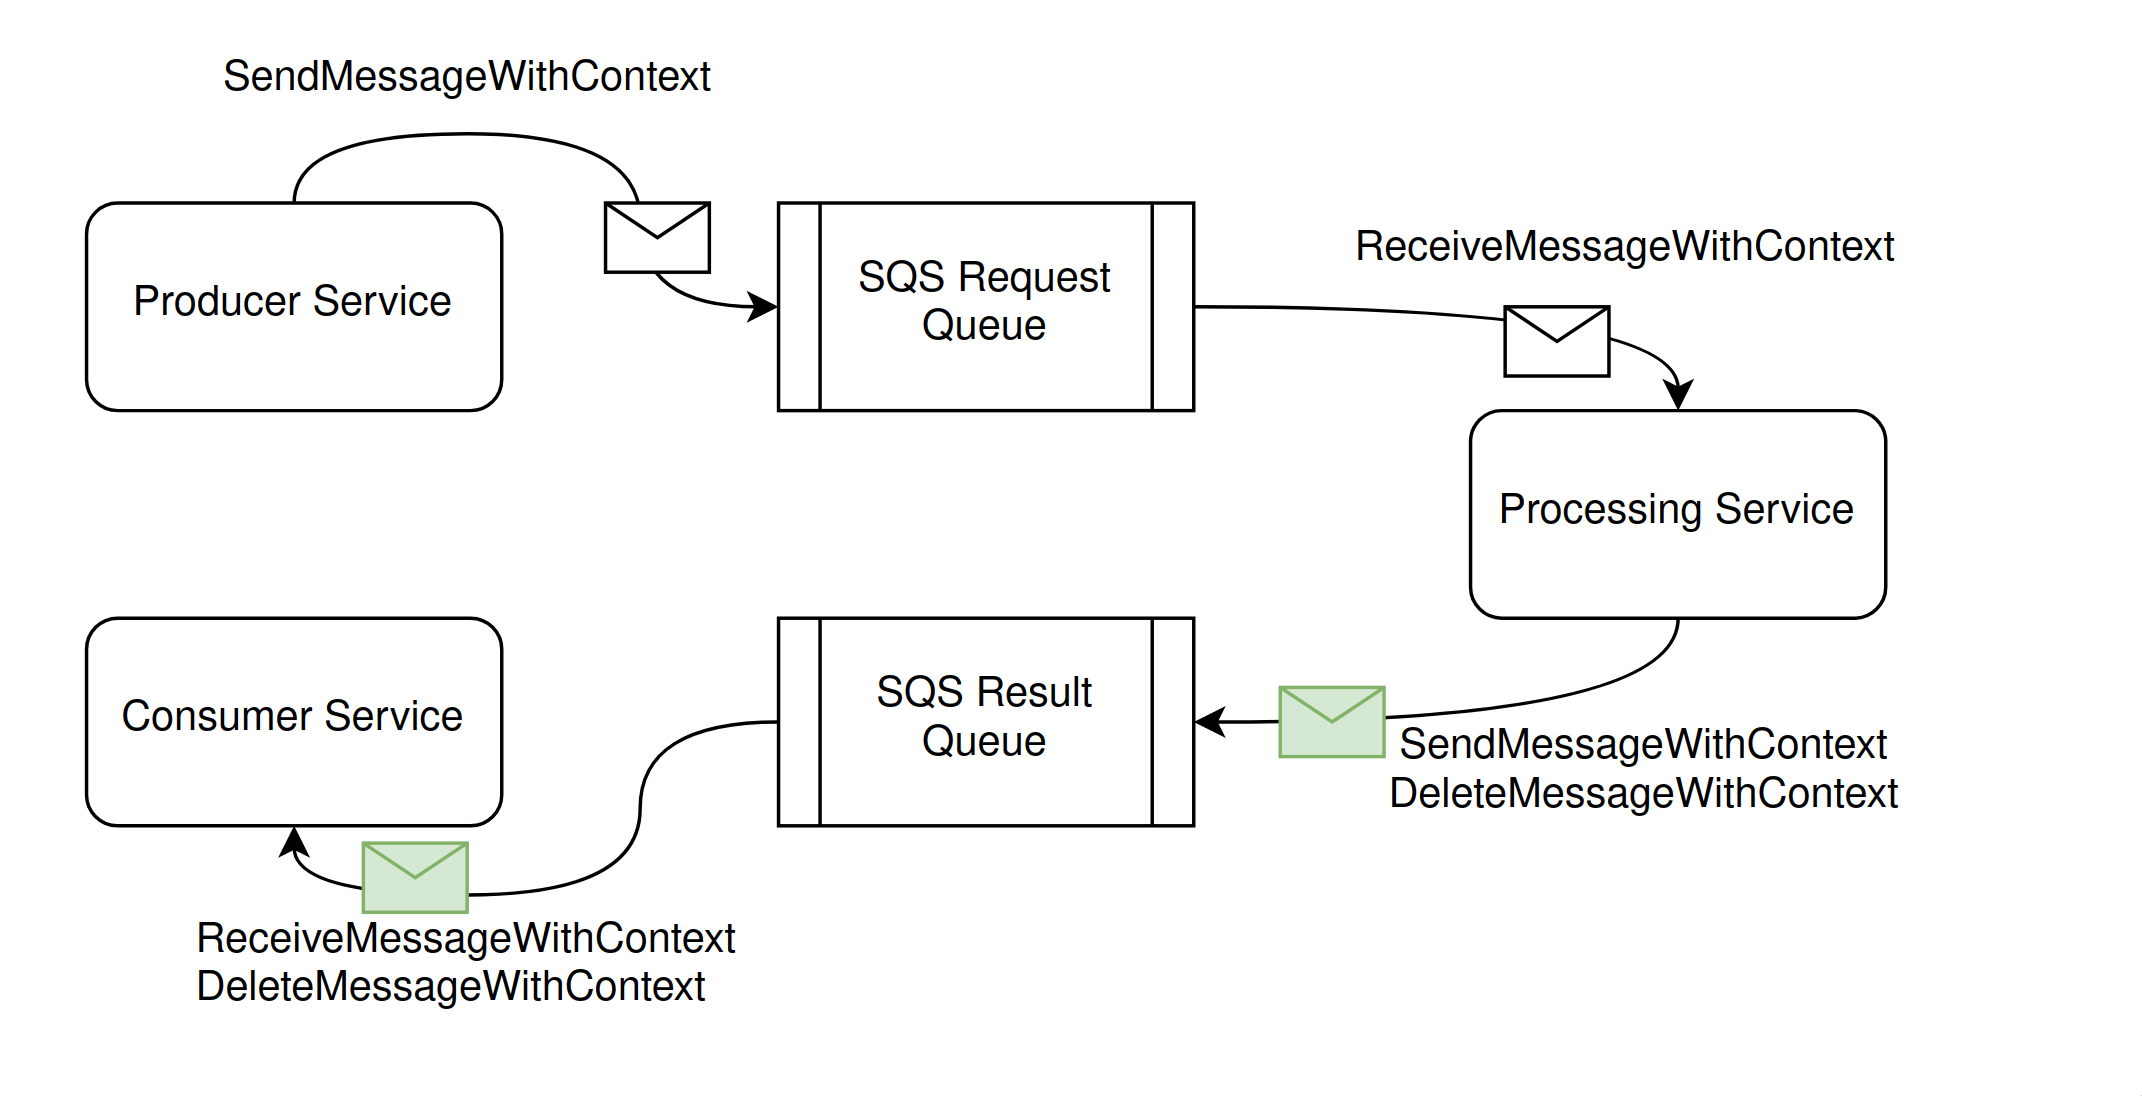
\includegraphics[width=0.95\textwidth]{img/sqs.png}
  \caption{SQS}
    \label{fig:sqs}
\end{figure}

\section{Вывод}
Из вышеперечисленного можно сделать вывод, что внедрение микросервисных практик не несет само по себе
каких-то однозначных преимуществ, а скорее является вынужденной мерой при развитии проектов и увеличении их кодовой базы.
В случае, когда:
\begin{enumerate}
    \item предприняты меры по анализу функций приложения для дальнейшего выделения
    логически независимых частей
    \item адаптированы общепринятые практики, связанные с развертыванием и оркестрацией сервисов, упрощающие 
    релизный цикл большого количества компонент
    \item налажены процессы тестирования и документации функциональности сервисов
    \item применяются stateless подходы к разработке сервисов и используются протоколы, обеспечивающие обратную совместимость
    \item уделено время по обеспечению консистентности данных в персистентных хранилищах
    \item используются механизмы кэширования, ретраев и балансировки для повышения надежности и снятия нагрузки сервисов
\end{enumerate}
Можно говорить о потенциальных преимуществах использования микросервисной архитектуры.
Исходя из количества мероприятий, которые требуются для эффективной эксплуатации распределенных систем,
стоит избегать деления на микросервисы в начале развития проекта, но проектировать системы,
имея в виду перспективы дальнейшего редизайна.

В случае перехода на микросервисную архитектуру зрелого приложения не стоит прерывать выстроенные процессы или пытаться
изменить архитектуру в рамках одной итерации. Подход, при котором изменения по разделению логики приложения распределяются
в отдельно развертываемые компоненты происходят инкрементально, называют переходом к удушающему приложению. Так проводится аналогия
с вьюном, который постепенно занимает все жизненное пространство. Аналогично первоначальный монолит распадается на отдельные микросервисы, пока
сам не становится микросервисом.